% Important: If latex complains about unicode characters,
% please use "\usepackage[utf8x]{inputenc}" in your preamble
% You can change the size of the picture by putting it into the construct:
% 1) \resizebox{10cm}{!}{"below picture"} to scale horizontally to 10 cm
% 2) \resizebox{!}{15cm}{"below picture"} to scale vertically to 15 cm
% 3) \resizebox{10cm}{15cm}{"below picture"} a combination of above two
% It is not recomended to use the scale option of the tikzpicture environment.
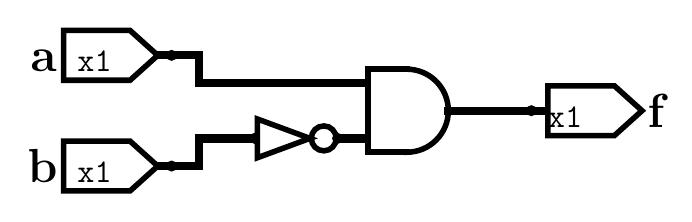
\begin{tikzpicture}[x=1pt,y=-1pt,line cap=rect]
\def\logisimfontA#1{\fontfamily{cmr}{#1}} % Replaced by logisim, original font was "SansSerif"
\def\logisimfontB#1{\fontfamily{cmtt}{#1}} % Replaced by logisim, original font was "Monospaced"
\definecolor{custcol_0_0_0}{RGB}{0, 0, 0}
\definecolor{custcol_ff_ff_ff}{RGB}{255, 255, 255}
\draw [line width=3.0pt, custcol_0_0_0 ]  (117.0,45.0) -- (127.0,45.0) ;
\draw [line width=3.0pt, custcol_0_0_0 ]  (157.0,35.0) -- (187.0,35.0) ;
\draw [line width=2.0pt, custcol_0_0_0] (142.0,50.0) arc (90.0:-90.0:15.0 and 15.0 );
\draw [line width=2.0pt, custcol_0_0_0 ]  (142.0,20.0) -- (128.0,20.0) -- (128.0,50.0) -- (142.0,50.0) ;
\draw [line width=2.0pt, custcol_0_0_0 ]  (107.0,45.0) -- (88.0,38.0) -- (88.0,52.0) -- cycle;
\draw [line width=2.0pt, custcol_0_0_0]  (112.0,45.0) ellipse (4.5 and 4.5 );
\fill [line width=2.0pt, custcol_0_0_0]  (117.0,45.0) ellipse (2.0 and 2.0 );
\fill [line width=2.0pt, custcol_0_0_0]  (87.0,45.0) ellipse (2.0 and 2.0 );
\draw [line width=3.0pt, custcol_0_0_0 ]  (52.0,55.0) -- (57.0,55.0) -- (67.0,55.0) -- (67.0,45.0) -- (87.0,45.0) ;
\draw [line width=2.0pt, custcol_0_0_0 ]  (42.0,64.0) -- (52.0,55.0) -- (42.0,46.0) -- (18.0,46.0) -- (18.0,64.0) -- cycle;
\logisimfontB{\fontsize{12pt}{12pt}\selectfont\node[inner sep=0, outer sep=0, custcol_0_0_0, anchor=base west] at  (23.0,61.0)  {x1};}
\logisimfontA{\fontsize{16pt}{16pt}\fontseries{bx}\selectfont\node[inner sep=0, outer sep=0, custcol_0_0_0, anchor=base west] at  (5.0,61.0)  {b};}
\fill [line width=2.0pt, custcol_0_0_0]  (57.0,55.0) ellipse (2.0 and 2.0 );
\draw [line width=3.0pt, custcol_0_0_0 ]  (52.0,15.0) -- (57.0,15.0) -- (67.0,15.0) -- (67.0,25.0) -- (127.0,25.0) ;
\draw [line width=2.0pt, custcol_0_0_0 ]  (42.0,24.0) -- (52.0,15.0) -- (42.0,6.0) -- (18.0,6.0) -- (18.0,24.0) -- cycle;
\logisimfontB{\fontsize{12pt}{12pt}\selectfont\node[inner sep=0, outer sep=0, custcol_0_0_0, anchor=base west] at  (23.0,21.0)  {x1};}
\logisimfontA{\fontsize{16pt}{16pt}\fontseries{bx}\selectfont\node[inner sep=0, outer sep=0, custcol_0_0_0, anchor=base west] at  (6.0,21.0)  {a};}
\fill [line width=2.0pt, custcol_0_0_0]  (57.0,15.0) ellipse (2.0 and 2.0 );
\draw [line width=3.0pt, custcol_0_0_0 ]  (191.0,35.0) -- (188.0,35.0) ;
\draw [line width=2.0pt, custcol_0_0_0 ]  (217.0,26.0) -- (227.0,35.0) -- (217.0,44.0) -- (193.0,44.0) -- (193.0,26.0) -- cycle;
\logisimfontB{\fontsize{12pt}{12pt}\selectfont\node[inner sep=0, outer sep=0, custcol_0_0_0, anchor=base west] at  (193.0,41.0)  {x1};}
\logisimfontA{\fontsize{16pt}{16pt}\fontseries{bx}\selectfont\node[inner sep=0, outer sep=0, custcol_0_0_0, anchor=base west] at  (229.0,41.0)  {f};}
\fill [line width=2.0pt, custcol_0_0_0]  (187.0,35.0) ellipse (2.0 and 2.0 );
\end{tikzpicture}

